% Copyright 2004 by Till Tantau <tantau@users.sourceforge.net>.
%
% In principle, this file can be redistributed and/or modified under
% the terms of the GNU Public License, version 2.
%
% However, this file is supposed to be a template to be modified
% for your own needs. For this reason, if you use this file as a
% template and not specifically distribute it as part of a another
% package/program, I grant the extra permission to freely copy and
% modify this file as you see fit and even to delete this copyright
% notice. 

\documentclass{beamer}

\usepackage{multirow}
\usepackage{color}
\usepackage{graphicx}
\usepackage{tikz}
\usetikzlibrary{trees,matrix}





% There are many different themes available for Beamer. A comprehensive
% list with examples is given here:
% http://deic.uab.es/~iblanes/beamer_gallery/index_by_theme.html
% You can uncomment the themes below if you would like to use a different
% one:
%\usetheme{AnnArbor}
%\usetheme{Antibes}
%\usetheme{Bergen}
%\usetheme{Berkeley}
%\usetheme{Berlin}
%\usetheme{Boadilla}
%\usetheme{boxes}
%\usetheme{CambridgeUS}
%\usetheme{Copenhagen}
%\usetheme{Darmstadt}
%\usetheme{default}
%\usetheme{Frankfurt}
%\usetheme{Goettingen}
%\usetheme{Hannover}
%\usetheme{Ilmenau}
%\usetheme{JuanLesPins}
%\usetheme{Luebeck}
\usetheme{Madrid}
%\usetheme{Malmoe}
%\usetheme{Marburg}
%\usetheme{Montpellier}
%\usetheme{PaloAlto}
%\usetheme{Pittsburgh}
%\usetheme{Rochester}
%\usetheme{Singapore}
%\usetheme{Szeged}
%\usetheme{Warsaw}


% remove navigation symbols
\setbeamertemplate{navigation symbols}{}

% Italic captions
\usepackage[textfont=it]{caption}

% small footnotes
\usepackage{setspace}



\title{Parallel Block Preconditioning of the Navier-Stokes Equations with
  Weakly Imposed Boundary Conditions}

\author{Raymon White}

% A subtitle is optional and this may be deleted
%\subtitle{Optional Subtitle}

% - Give the names in the same order as the appear in the paper.
% - Use the \inst{?} command only if the authors have different
%   affiliation.

%\institute[Universities of Somewhere and Elsewhere] % (optional, but mostly needed)
%{
%  \inst{1}%
%  Department of Computer Science\\
%  University of Somewhere
%  \and
%  \inst{2}%
%  Department of Theoretical Philosophy\\
%  University of Elsewhere}
%% - Use the \inst command only if there are several affiliations.
%% - Keep it simple, no one is interested in your street address.
%
%\date{Conference Name, 2013}
%% - Either use conference name or its abbreviation.
%% - Not really informative to the audience, more for people (including
%%   yourself) who are reading the slides online
%
%\subject{Theoretical Computer Science}
% This is only inserted into the PDF information catalog. Can be left
% out. 

% If you have a file called "university-logo-filename.xxx", where xxx
% is a graphic format that can be processed by latex or pdflatex,
% resp., then you can add a logo as follows:

% \pgfdeclareimage[height=0.5cm]{university-logo}{university-logo-filename}
% \logo{\pgfuseimage{university-logo}}

% Delete this, if you do not want the table of contents to pop up at
% the beginning of each subsection:
%\AtBeginSubsection[]
%{
%  \begin{frame}<beamer>{Outline}
%    \tableofcontents[currentsection,currentsubsection]
%  \end{frame}
%}

% Let's get started
\begin{document}

\begin{frame}
  \titlepage
\end{frame}

%\begin{frame}{Outline}
%  \tableofcontents
%  % You might wish to add the option [pausesections]
%\end{frame}


\newcommand{\vsol}{\psi}
\newcommand{\ijdim}{\text{for } i,j = 1,2\,[,3]}
\newcommand{\psol}{\varphi}
\newcommand{\idim}{\text{for } i = 1,2\,[,3]}

\begin{frame} \frametitle{Overall goal}
Goal: Develop a (new) preconditioning algorithm for the
      Navier-Stokes equations with boundary conditions imposed via Lagrange 
      Multiplier constraints.

\begin{itemize}%[noitemsep,topsep=0pt]
\item Constrained Navier-Stokes equations (in residual form):
\begin{align}
	r_{i}^{(u)}=&\int_\Omega \left[ Re\; \left( St\frac{\partial u_i}{\partial t}+ u_j \frac{\partial
    u_i}{\partial x_j} \right)    \vsol{} + \tau_{ij}\frac{\partial
  \vsol{}}{\partial x_j} \right]  \,\mathrm{d}\Omega \nonumber\\
   	& + \delta \int_{\partial \Omega_c} \lambda u_i c_i \,\mathrm{d}S = 0,
    \quad \ijdim,	\label{eq:nsweakform_stated2} \\
r^{(p)}=&\int_{\Omega}\left( \frac{\partial u_i}{\partial x_i} - Q
\right)\psol{}	\,\mathrm{d}\Omega = 0, \quad \idim.
\label{eq:continweakform_stated2} \\
 r^{(\lambda)} = &\delta \int_{\partial \Omega_c} \lambda u_i c_i
 \,\mathrm{d}S = 0,  \quad \idim.\label{eq:lgrweakform} 
\end{align}
\end{itemize}
\end{frame}

%%%%%%%%%%%%%%%%%%%%%%%%%%%%%%%%%%%%%%%%%%%%%%%%%%%%%%%%%%%%%%%%%%%%%%%%%%%%
\newcommand{\genjac}{\mathcal{F}}
\newcommand{\nsjac}{F_{NS}}
\begin{frame}

\begin{itemize}
\item Block structure of Jacobian:
\begin{equation*}
\genjac = 
  \begin{bmatrix}
    F & B^T & \widehat{L}^T\\
    B & \mathit{O} & \mathit{O} \\
    \widehat{L} & \mathit{O} & \mathit{O}
  \end{bmatrix}
\begin{array}{c}
 \updownarrow n_u\\ 
 \updownarrow n_p\\
 \updownarrow n_l\\
\end{array}
\quad \mbox{and} \quad
\end{equation*}
\item Preconditioner:
\begin{equation*}
\mathcal{P} = 
  \begin{bmatrix}
    F + \widehat{L}^T\,(\frac{1}{\sigma}\widehat{L}\widehat{L}^T)^{-1}\,\widehat{L}& B^T & \mathit{O}\\
    B & \mathit{O} & \mathit{O} \\
    \mathit{O} & \mathit{O} & \frac{1}{\sigma}\widehat{L}\widehat{L}^T
  \end{bmatrix}
\begin{array}{c}
 \updownarrow n_u\\ 
 \updownarrow n_p\\
 \updownarrow n_l\\
\end{array}
\end{equation*}
\begin{itemize} 
\item $\widehat{L}$ - Lagrange multiplier block matrix.
\end{itemize}
\item For $\mathcal{F}v = \mu\mathcal{P}v$, analytical proof that for
  Reynolds number $Re = 0$,
  \begin{itemize}
  \item  $\sigma = ||F||_{\infty} \implies 
  \mu = \begin{cases}
   1   & \times (n_u + n_p) \\
   [-1,-\frac{1}{3}]  & \times n_l
  \end{cases} $
  \end{itemize}
\end{itemize}
\end{frame}


%%%%%%%%%%%%%%%%%%%%%%%%%%%%%%%%%%%%%%%%%%%%%%%%%%%%%%%%%%%%%%%%%%%%%%%%%%%%
\begin{frame} \frametitle{Block Preconditioning Framework (BPF)}
Overview:
\begin{itemize}
  \item Software (middleware) that facilitates rapid development of problem
    specific block preconditioners.
  \item Hides low-level implementation details (including parallelisation)
    from the expert user.
  \item Block preconditioning can lead to the development of optimal solvers
    for a number of important problem classes.
    % Linear elasticity, electromagnetics, micromagnetics, NS-equations,
    % multiphysics problems.

\end{itemize}
\end{frame}

%%%%%%%%%%%%%%%%%%%%%%%%%%%%%%%%%%%%%%%%%%%%%%%%%%%%%%%%%%%%%%%%%%%%%%%%%%%%
\begin{frame} \frametitle{Block Preconditioning Framework (BPF)}
Overview:
\begin{itemize}
  \item The BPF is based on two design premises:
    \begin{itemize}
      \item A block preconditioner can be one of three types: block
        diagonal, upper/lower block triangular.
      \item The approximate inversion of the principal diagonal blocks is
        either achieved by recursive application of the definition of the
        preconditioner or by iterative scalar solvers such as multigrid. % such as multi grid
      \end{itemize}

  \item Recursive definition allows complex preconditioners to be
    represented as a tree structure (re-use of existing block
    preconditioners).
\end{itemize}
\end{frame}


%%%%%%%%%%%%%%%%%%%%%%%%%%%%%%%%%%%%%%%%%%%%%%%%%%%%%%%%%%%%%%%%%%%%%%%%%%%%
\begin{frame} \frametitle{Block Preconditioning Hierarchy}
\begin{figure}[H]
    \centering
    \includegraphics[trim = 1mm 1mm 1mm 1mm,clip,width=0.9\textwidth]{./pic/bpf_hierarchy_matrixstructure.pdf}
\end{figure}
\end{frame}

%%%%%%%%%%%%%%%%%%%%%%%%%%%%%%%%%%%%%%%%%%%%%%%%%%%%%%%%%%%%%%%%%%%%%%%%%%%%
\begin{frame} \frametitle{Blocking functionality}
Classification of degrees of freedom at element level:
\newline
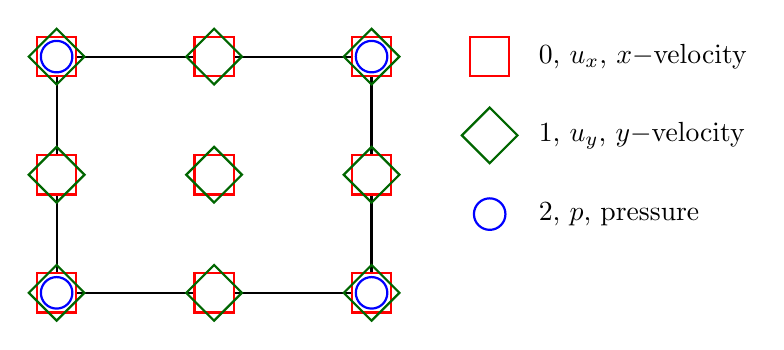
\begin{tikzpicture}
%\draw[help lines] (0,0) grid (10,3);

% Define the points on the square
\pgfmathsetmacro{\Xleft}{0};
\pgfmathsetmacro{\Xmid}{2};
\pgfmathsetmacro{\Xright}{4};
\pgfmathsetmacro{\Ybot}{0};
\pgfmathsetmacro{\Ymid}{1.5};
\pgfmathsetmacro{\Ytop}{3};

% draw the element outline
\draw [thick](\Xleft,\Ybot) -- (\Xleft,\Ytop) 
             -- (\Xright,\Ytop) -- (\Xright,\Ybot) -- (\Xleft,\Ybot);

% Draw the velocity nodes
\pgfmathsetmacro{\Shapesize}{0.25};
\draw [red,thick,fill=white] (\Xleft-\Shapesize,\Ybot-\Shapesize) rectangle (\Xleft+\Shapesize,\Ybot+\Shapesize);
\draw [red,thick,fill=white] (\Xmid-\Shapesize,\Ybot-\Shapesize) rectangle (\Xmid+\Shapesize,\Ybot+\Shapesize);
\draw [red,thick,fill=white] (\Xright-\Shapesize,\Ybot-\Shapesize) rectangle (\Xright+\Shapesize,\Ybot+\Shapesize);
\draw [red,thick,fill=white] (\Xleft-\Shapesize,\Ymid-\Shapesize) rectangle (\Xleft+\Shapesize,\Ymid+\Shapesize);
\draw [red,thick,fill=white] (\Xmid-\Shapesize,\Ymid-\Shapesize) rectangle (\Xmid+\Shapesize,\Ymid+\Shapesize);
\draw [red,thick,fill=white] (\Xright-\Shapesize,\Ymid-\Shapesize) rectangle (\Xright+\Shapesize,\Ymid+\Shapesize);
\draw [red,thick,fill=white] (\Xleft-\Shapesize,\Ytop-\Shapesize)rectangle (\Xleft+\Shapesize,\Ytop+\Shapesize);
\draw [red,thick,fill=white] (\Xmid-\Shapesize,\Ytop-\Shapesize) rectangle(\Xmid+\Shapesize,\Ytop+\Shapesize);
\draw [red,thick,fill=white] (\Xright-\Shapesize,\Ytop-\Shapesize) rectangle (\Xright+\Shapesize,\Ytop+\Shapesize);


\draw [black!60!green,rotate=45,thick] (\Xleft-\Shapesize,\Ybot-\Shapesize) rectangle (\Xleft+\Shapesize,\Ybot+\Shapesize);
\draw [black!60!green,rotate around={45:(\Xmid,\Ybot)},thick] (\Xmid-\Shapesize,\Ybot-\Shapesize) rectangle (\Xmid+\Shapesize,\Ybot+\Shapesize);
\draw [black!60!green,rotate around={45:(\Xright,\Ybot)},thick] (\Xright-\Shapesize,\Ybot-\Shapesize) rectangle (\Xright+\Shapesize,\Ybot+\Shapesize);
\draw [black!60!green,rotate around={45:(\Xleft,\Ymid)},thick] (\Xleft-\Shapesize,\Ymid-\Shapesize) rectangle (\Xleft+\Shapesize,\Ymid+\Shapesize);
\draw [black!60!green,rotate around={45:(\Xmid,\Ymid)},thick] (\Xmid-\Shapesize,\Ymid-\Shapesize) rectangle (\Xmid+\Shapesize,\Ymid+\Shapesize);
\draw [black!60!green,rotate around={45:(\Xright,\Ymid)},thick] (\Xright-\Shapesize,\Ymid-\Shapesize) rectangle (\Xright+\Shapesize,\Ymid+\Shapesize);
\draw [black!60!green,rotate around={45:(\Xleft,\Ytop)},thick] (\Xleft-\Shapesize,\Ytop-\Shapesize)rectangle (\Xleft+\Shapesize,\Ytop+\Shapesize);
\draw [black!60!green,rotate around={45:(\Xmid,\Ytop)},thick] (\Xmid-\Shapesize,\Ytop-\Shapesize) rectangle(\Xmid+\Shapesize,\Ytop+\Shapesize);
\draw [black!60!green,rotate around={45:(\Xright,\Ytop)},thick] (\Xright-\Shapesize,\Ytop-\Shapesize) rectangle (\Xright+\Shapesize,\Ytop+\Shapesize);


\draw [blue,thick] (\Xleft,\Ybot) circle [radius=0.2];
\draw [blue,thick] (\Xright,\Ybot) circle [radius=0.2];
\draw [blue,thick] (\Xleft,\Ytop) circle [radius=0.2];
\draw [blue,thick] (\Xright,\Ytop) circle [radius=0.2];

%%%%%%%%%%%%%%%%%%%%%%%%%%%%%%%%%%%%%%%%%%%%%%%%%%%%%%%%%%%%%%%%%%%%%%%%%%%%
\draw [red,thick,fill=white] (5.5-\Shapesize,3-\Shapesize)rectangle(5.5+\Shapesize,3+\Shapesize);
\node[anchor=west] at (6,3) {$0$, $u_x$, $x-$velocity};

\draw [black!60!green,rotate around={45:(5.5,2)},thick] (5.5-\Shapesize,2-\Shapesize) rectangle (5.5+\Shapesize,2+\Shapesize);
\node[anchor=west] at (6,2) {$1$, $u_y$, $y-$velocity};

\draw [blue,thick] (5.5,1) circle [radius=0.2];
\node[anchor=west] at (6,1) {$2$, $p$, pressure};
\end{tikzpicture}
\begin{tabular}{c|c|c|c|c|c|c|c|c|c|c|}
\cline{2-10}
                                 & $u_x$ &$u_y$ & $p$ & $u_x$ & $u_y$ & $u_x$ & $u_y$ & $p$ &$\ldots$ \\ 
\cline{1-10}
\multicolumn{1}{ |c| }{$G_i$}    & 0     & 1    & 2   & 3     & 4     &  5    &  6    & 7  & $\ldots$\\ 
\cline{1-10}
\multicolumn{1}{ |c| }{Dof type} & 0     & 1    & 2   & 0     & 1     &  0    &  1    & 2 & $\ldots$\\ 
\cline{1-10}
\end{tabular}
\end{frame}

%%%%%%%%%%%%%%%%%%%%%%%%%%%%%%%%%%%%%%%%%%%%%%%%%%%%%%%%%%%%%%%%%%%%%%%%%%%%
\begin{frame} \frametitle{Blocking}

\begin{equation*}
\underbrace{
  \begin{bmatrix}
           &   &  \\
           \quad        & \scalebox{3}{$ F$}  & \quad \\
           &   &    
  \end{bmatrix}
}_\text{Natural ordered Jacobian}
\rightarrow
\underbrace{
  \begin{bmatrix}
    F_{xx} & F_{xy} & B_{x}^{T} \\
    F_{yx} & F_{yy} & B_{y}^{T} \\
    B_{x}  & B_{y}  &       
  \end{bmatrix}
}_{\substack{\text{Dof type blocking}\\\text{(Dof-blocks)}}}
\rightarrow
\underbrace{
  \begin{bmatrix}
   \scalebox{2}{$F$} &\scalebox{2}{$ B^{T}$} \\
   \scalebox{2}{$B$} &         
  \end{bmatrix}
}_\text{Concatenation of dof-blocks}
\end{equation*}

\begin{equation*}
\underbrace{
  \begin{bmatrix}
           &   &  \\
           \quad        & \scalebox{3}{$ F$}  & \quad \\
           &   &    
  \end{bmatrix}
}_\text{Natural ordered Jacobian}
\rightarrow
\underbrace{
  \begin{bmatrix}
    \color{red}{\tilde{F}_{xx}} & F_{xy} & B_{x}^{T} \\
    F_{yx} & \color{red}{\tilde{F}_{yy}} & B_{y}^{T} \\
    B_{x}  & B_{y}  &       
  \end{bmatrix}
}_\text{Replacement of dof-blocks}
\rightarrow
\underbrace{
  \begin{bmatrix}
   \scalebox{2}{\color{red}{$\tilde{F}$}} &\scalebox{2}{$ B^{T}$} \\
   \scalebox{2}{$B$} &         
  \end{bmatrix}
}_{\substack{\text{Concatenated dof-block}\\\text{(with replacement)}}}
\end{equation*}
\end{frame}


%%%%%%%%%%%%%%%%%%%%%%%%%%%%%%%%%%%%%%%%%%%%%%%%%%%%%%%%%%%%%%%%%%%%%%%%%%%%
\begin{frame} \frametitle{Parallel results for 3D annular wedge}
\begin{figure}[H]
    \centering
    \includegraphics[trim = 1mm 1mm 1mm 1mm, clip,width=0.5\textwidth]{./pic/annularwedge3d.eps}
    \caption{Plot of the solution for the unsteady uniform radial flow
      through an annulus wedge with $Re$ = 100 at
      time $t = 0.3$. The contour and streamlines represent the pressure
      gradient and velocity flow field respectively.}
    \label{fig:annularwedge3d}
\end{figure}
\end{frame}

%%%%%%%%%%%%%%%%%%%%%%%%%%%%%%%%%%%%%%%%%%%%%%%%%%%%%%%%%%%%%%%%%%%%%%%%%%%%
\begin{frame}\frametitle{Preconditioning algorithm}
Preconditioner: Inexact LSC Augmented Preconditioner
\begin{itemize}
  \item Block Diagonal Preconditioner
    \begin{itemize}
      \item{Navier-Stokes Preconditioner:} LSC
        \begin{itemize}
          \item{Momentum Preconditioner:} BoomerAMG \\
           V-cycles: 1v22 \\ 
           Coarsening strategy: Falgout / PMIS \\
           Strength of dependence 0.75 \\
           Smoother: SOR 
          \item{Pressure Schur Complement Preconditioner:} BoomerAMG \\
           V-cycles: 1v22 \\
           Coarsening strategy: Falgout \\
           Strength of dependence: 0.7 \\
           Smoother: SOR \\
          \end{itemize}

      \item{W-block Preconditioner:} SuperLU
      \end{itemize}
  \end{itemize}
  Intel CPU: 12 cores: 1 node with two 6-core Xeon X7542 2.67GHz (Westmere, SSE4.2)
\end{frame}


%%%%%%%%%%%%%%%%%%%%%%%%%%%%%%%%%%%%%%%%%%%%%%%%%%%%%%%%%%%%%%%%%%%%%%%%%%%%
\begin{frame}\frametitle{Weak scaling results}
Falgout coarsening for the momentum block
\begin{center}
  \begin{tabular}{| c | c | c | c | c | c|}
    \hline
    No. Proc      &    1     &    2  &  4     & 8     & 16  \\ \hline
    No. Dof       & 70717    &149313 &271461  &557343 &1180551 \\ \hline
    Jacobian      & 9.63     &13.90  &15.01   &17.52  &15.00 \\ \hline
    Prec.         &3.61	     &6.89   &11.92   &15.58  &19.48 \\ \hline
    BPF           &3.47      &9.14   &11.03   &16.31  &22.77 \\ \hline
    Krylov solve  &11.89     &15.47  &19.32   &29.30  &34.70 \\ \hline
    Iterations    &30.27     &28.7   &28.9    &29.17  &30.8  \\
    \hline
    \end{tabular}
\end{center}
\end{frame}

%%%%%%%%%%%%%%%%%%%%%%%%%%%%%%%%%%%%%%%%%%%%%%%%%%%%%%%%%%%%%%%%%%%%%%%%%%%%
\begin{frame}\frametitle{Weak scaling results}
PMIS coarsening for the momentum block
\begin{center}
  \begin{tabular}{| c | c | c | c | c | c|}
    \hline
    No. Proc      &    1     &    2  &  4     & 8     & 16  \\ \hline
    No. Dof       & 70717    &149313 &271461  &557343 &1180551 \\ \hline
    Jacobian      &9.62      &13.90  &14.92   &17.65  &14.98 \\ \hline
    Prec.         &2.35      &3.33   &4.81    &6.87   &8.79 \\ \hline
    BPF           &3.48	     &9.10   &11.19   &16.45  &22.99 \\ \hline
    Krylov        &7.86	     &9.73   &11.57   &17.79  &20.88 \\ \hline
    Iterations    &31.13     &29.77  &30.23   &29.66  &31.28\\
    \hline
    \end{tabular}
\end{center}
\end{frame}


%%%%%%%%%%%%%%%%%%%%%%%%%%%%%%%%%%%%%%%%%%%%%%%%%%%%%%%%%%%%%%%%%%%%%%%%%%%%
\begin{frame}\frametitle{Break down of BPF}

 Break down of BPF overhead from PMIS times:
\begin{center}
  \begin{tabular}{| c | c | c | c | c|}
    \hline
    No. Proc      &    2  &  4     & 8     & 16  \\ \hline
    No. Dof       &149313 &271461  &557343 &1180551 \\ \hline
    Master block\_setup(...)  &0.76   &2.28    &6.27   &12.23 \\ \hline
    Other  (e.g. get\_block(...))    &8.34   &8.91    &10.19  &10.77 \\
    \hline
    \end{tabular}
\end{center}
\end{frame}
%%%%%%%%%%%%%%%%%%%%%%%%%%%%%%%%%%%%%%%%%%%%%%%%%%%%%%%%%%%%%%%%%%%%%%%%%%%%
\begin{frame}\frametitle{Summary}
  \begin{itemize}
\item Developed an optimal preconditioner for an important problem class of the Navier-Stokes equations.
\item Significant functional upgrade of the parallel general block preconditioning framework.
\item Good parallel scaling observed.
\end{itemize}
\end{frame}







% Section and subsections will appear in the presentation overview
% and table of contents.
\section{First Main Section}

\subsection{First Subsection}

\begin{frame}{First Slide Title}{Optional Subtitle}
  \begin{itemize}
  \item {
    My first point.
  }
  \item {
    My second point.
  }
  \end{itemize}
\end{frame}

\subsection{Second Subsection}

% You can reveal the parts of a slide one at a time
% with the \pause command:
\begin{frame}{Second Slide Title}
  \begin{itemize}
  \item {
    First item.
    \pause % The slide will pause after showing the first item
  }
  \item {   
    Second item.
  }
  % You can also specify when the content should appear
  % by using <n->:
  \item<3-> {
    Third item.
  }
  \item<4-> {
    Fourth item.
  }
  % or you can use the \uncover command to reveal general
  % content (not just \items):
  \item<5-> {
    Fifth item. \uncover<6->{Extra text in the fifth item.}
  }
  \end{itemize}
\end{frame}

\section{Second Main Section}

\subsection{Another Subsection}

\begin{frame}{Blocks}
\begin{block}{Block Title}
You can also highlight sections of your presentation in a block, with it's own title
\end{block}
\begin{theorem}
There are separate environments for theorems, examples, definitions and proofs.
\end{theorem}
\begin{example}
Here is an example of an example block.
\end{example}
\end{frame}

% Placing a * after \section means it will not show in the
% outline or table of contents.
\section*{Summary}

\begin{frame}{Summary}
  \begin{itemize}
  \item
    The \alert{first main message} of your talk in one or two lines.
  \item
    The \alert{second main message} of your talk in one or two lines.
  \item
    Perhaps a \alert{third message}, but not more than that.
  \end{itemize}
  
  \begin{itemize}
  \item
    Outlook
    \begin{itemize}
    \item
      Something you haven't solved.
    \item
      Something else you haven't solved.
    \end{itemize}
  \end{itemize}
\end{frame}



% All of the following is optional and typically not needed. 
\appendix
\section<presentation>*{\appendixname}
\subsection<presentation>*{For Further Reading}

\begin{frame}[allowframebreaks]
  \frametitle<presentation>{For Further Reading}
    
  \begin{thebibliography}{10}
    
  \beamertemplatebookbibitems
  % Start with overview books.

  \bibitem{Author1990}
    A.~Author.
    \newblock {\em Handbook of Everything}.
    \newblock Some Press, 1990.
 
    
  \beamertemplatearticlebibitems
  % Followed by interesting articles. Keep the list short. 

  \bibitem{Someone2000}
    S.~Someone.
    \newblock On this and that.
    \newblock {\em Journal of This and That}, 2(1):50--100,
    2000.
  \end{thebibliography}
\end{frame}

\end{document}


